% Options for packages loaded elsewhere
\PassOptionsToPackage{unicode}{hyperref}
\PassOptionsToPackage{hyphens}{url}
%
\documentclass[
  ignorenonframetext,
]{beamer}
\usepackage{pgfpages}
\setbeamertemplate{caption}[numbered]
\setbeamertemplate{caption label separator}{: }
\setbeamercolor{caption name}{fg=normal text.fg}
\beamertemplatenavigationsymbolsempty
% Prevent slide breaks in the middle of a paragraph
\widowpenalties 1 10000
\raggedbottom
\setbeamertemplate{part page}{
  \centering
  \begin{beamercolorbox}[sep=16pt,center]{part title}
    \usebeamerfont{part title}\insertpart\par
  \end{beamercolorbox}
}
\setbeamertemplate{section page}{
  \centering
  \begin{beamercolorbox}[sep=12pt,center]{section title}
    \usebeamerfont{section title}\insertsection\par
  \end{beamercolorbox}
}
\setbeamertemplate{subsection page}{
  \centering
  \begin{beamercolorbox}[sep=8pt,center]{subsection title}
    \usebeamerfont{subsection title}\insertsubsection\par
  \end{beamercolorbox}
}
\AtBeginPart{
  \frame{\partpage}
}
\AtBeginSection{
  \ifbibliography
  \else
    \frame{\sectionpage}
  \fi
}
\AtBeginSubsection{
  \frame{\subsectionpage}
}
\usepackage{amsmath,amssymb}
\usepackage{iftex}
\ifPDFTeX
  \usepackage[T1]{fontenc}
  \usepackage[utf8]{inputenc}
  \usepackage{textcomp} % provide euro and other symbols
\else % if luatex or xetex
  \usepackage{unicode-math} % this also loads fontspec
  \defaultfontfeatures{Scale=MatchLowercase}
  \defaultfontfeatures[\rmfamily]{Ligatures=TeX,Scale=1}
\fi
\usepackage{lmodern}
\ifPDFTeX\else
  % xetex/luatex font selection
\fi
% Use upquote if available, for straight quotes in verbatim environments
\IfFileExists{upquote.sty}{\usepackage{upquote}}{}
\IfFileExists{microtype.sty}{% use microtype if available
  \usepackage[]{microtype}
  \UseMicrotypeSet[protrusion]{basicmath} % disable protrusion for tt fonts
}{}
\makeatletter
\@ifundefined{KOMAClassName}{% if non-KOMA class
  \IfFileExists{parskip.sty}{%
    \usepackage{parskip}
  }{% else
    \setlength{\parindent}{0pt}
    \setlength{\parskip}{6pt plus 2pt minus 1pt}}
}{% if KOMA class
  \KOMAoptions{parskip=half}}
\makeatother
\usepackage{xcolor}
\newif\ifbibliography
\usepackage{graphicx}
\makeatletter
\newsavebox\pandoc@box
\newcommand*\pandocbounded[1]{% scales image to fit in text height/width
  \sbox\pandoc@box{#1}%
  \Gscale@div\@tempa{\textheight}{\dimexpr\ht\pandoc@box+\dp\pandoc@box\relax}%
  \Gscale@div\@tempb{\linewidth}{\wd\pandoc@box}%
  \ifdim\@tempb\p@<\@tempa\p@\let\@tempa\@tempb\fi% select the smaller of both
  \ifdim\@tempa\p@<\p@\scalebox{\@tempa}{\usebox\pandoc@box}%
  \else\usebox{\pandoc@box}%
  \fi%
}
% Set default figure placement to htbp
\def\fps@figure{htbp}
\makeatother
\setlength{\emergencystretch}{3em} % prevent overfull lines
\providecommand{\tightlist}{%
  \setlength{\itemsep}{0pt}\setlength{\parskip}{0pt}}
\setcounter{secnumdepth}{-\maxdimen} % remove section numbering
%\logo{
\includegraphics[height=1.2cm,width=3cm]{logo.jpg}} % use this if you want logo.jpg on every slide
\usepackage{tabulary}
\usepackage{tablefootnote}
\usepackage{threeparttable}

\usetheme{Ilmenau}
%\usecolortheme{spruce} %can comment out the rest and use the basic color theme
\institute{Canadian Research Data Centre Network}{Réseau Canadien Des Centres De Données De Recherche}
\setbeamertemplate{navigation symbols}{}

\titlegraphic{
\includegraphics[height=1.8cm,width=3.27cm]{content/logo.png}} %those numbers keep the aspect ratio of the original (1/.55)

%colors can be put into the presentation below. For mcmaster colors use uncomment A, for a three color school uncomment B, and for a two color school uncomment C 

%three color school input
%Current: CRDCN
\definecolor{primco}{HTML}{527CA6}
\definecolor{secondco}{HTML}{E1E3E4}
\definecolor{tertco}{HTML}{1F516E}

%two color school input
%Current: mount royal
%\definecolor{color1}{RGB}{21,71,52} 
%\definecolor{color2}{RGB}{192,181,97}

%McMaster official colors
%\definecolor{color1}{HTML}{990033}
%\definecolor{color2}{HTML}{666666}

%A - Uncomment this section for mcmaster Colors
%setbeamercolor{frametitle}{fg=macmar,bg=white}
%setbeamercolor{title}{fg=macslv,bg=white}
%setbeamercolor{structure}{fg=macmar}
%setbeamercolor{local structure}{fg=macmar}
%setbeamercolor{section in toc}{fg=macmar,bg=macslv}
%setbeamercolor{subsection in toc}{fg=macmar,bg=macslv}

%setbeamercolor{item projected}{fg=macmar,bg=macslv}
%setbeamertemplate{itemize item}{\color{macmar}$\bullet$}
%setbeamertemplate{itemize subitem}{\color{macslv}\scriptsize{$\bullet$}}
%setbeamertemplate{itemize subsubitem}{\color{macslv}\scriptsize{$\bullet$}}
%setbeamertemplate{}


%B - Uncomment this section for Guest presenter colors for a three color school
\setbeamercolor{frametitle}{fg=primco,bg=secondco}
\setbeamercolor{title}{fg=primco,bg=white}
\setbeamercolor{structure}{fg=primco}
\setbeamercolor{local structure}{fg=secondco}
\setbeamercolor{section in toc}{fg=secondco,bg=tertco}

\setbeamercolor{subsection in toc}{fg=primco,bg=tertco}

\setbeamercolor{item projected}{fg=secondco,bg=primco}
\setbeamertemplate{itemize item}{\color{primco}$\bullet$}
\setbeamertemplate{itemize subitem}{\color{secondco}\scriptsize{$\bullet$}}
\setbeamertemplate{itemize subsubitem}{\color{tertco}\scriptsize{$\bullet$}}
\setbeamertemplate{}


%C - Uncomment this section for Guest presenter colors for a two color school
%\setbeamercolor{frametitle}{fg=color1,bg=white}
%\setbeamercolor{title}{fg=color2,bg=white}
%\setbeamercolor{structure}{fg=color1}
%\setbeamercolor{local structure}{fg=color1}
%\setbeamercolor{section in toc}{fg=color1,bg=color2}

%\setbeamercolor{subsection in toc}{fg=color1,bg=color2}

%\setbeamercolor{item projected}{fg=color2,bg=color1}
%\setbeamercolor{subitem projected}{fg=color2,bg=color1}
%\setbeamertemplate{itemize item}{\color{color1}$\bullet$}
%\setbeamertemplate{itemize subitem}{\color{color2}\scriptsize{$\bullet$}}
%\setbeamertemplate{itemize subsubitem}{\color{color2}\scriptsize{$\bullet$}}
%\setbeamertemplate{}

\usepackage{hyperref}
\hypersetup{
    colorlinks=true,
    linkcolor=yellow,    % color of internal links
    filecolor=red, % color of file links
    urlcolor=blue,     % color of external links
    citecolor=purple,   % color of citation links
}
\usepackage{bookmark}
\IfFileExists{xurl.sty}{\usepackage{xurl}}{} % add URL line breaks if available
\urlstyle{same}
\hypersetup{
  pdftitle={Portes ouvertes aux données},
  pdfauthor={Grant Gibson},
  hidelinks,
  pdfcreator={LaTeX via pandoc}}

\title{Portes ouvertes aux données}
\author{Grant Gibson}
\date{Date: 2025-08-27}

\begin{document}
\frame{\titlepage}

\begin{frame}{Introduction}
\phantomsection\label{introduction}
\begin{itemize}
\tightlist
\item
  Merci au CRSH pour son soutien au projet « Portes ouvertes aux données
  » dans le cadre du programme Connexion, volet GDR.
\item
  Merci au RCCDR et à ses bailleurs de fonds : la FCI, les IRSC, le
  CRSH, les partenaires provinciaux et les institutions collaboratrices.
\end{itemize}

Merci d'accéder au dossier du projet pour cet atelier :
www.github.com/CRDCN/RAD\_training
\end{frame}

\begin{frame}{Introduction}
\phantomsection\label{introduction-1}
\begin{itemize}
\tightlist
\item
  Évolution de la découvrabilité des données et de la science ouverte
\item
  Pressions exercées pas les revues scientifiques
\item
  Pressions exercées par les conseils
\item
  Pressions au sein des universités
\end{itemize}
\end{frame}

\begin{frame}{Pour contenir la séance}
\phantomsection\label{pour-contenir-la-suxe9ance}
\begin{itemize}
\tightlist
\item
  Aujourd'hui, nous parlons des données à accès restreint
\item
  Il ne s'agit pas de toutes les données sensibles, ni de données
  ouvertes, mais de données assorties d'un processus ou d'un mécanisme
  d'accès
\end{itemize}
\end{frame}

\begin{frame}{Objectifs}
\phantomsection\label{objectifs}
\begin{itemize}
\tightlist
\item
  Données FAIR
\item
  « Aussi ouvertes que possible, aussi fermées que nécessaire »
\item
  Ce n'est pas un choix binaire, mais d'un continuum
\end{itemize}
\end{frame}

\begin{frame}{Contibutions des chercheurs à FAIR}
\phantomsection\label{contibutions-des-chercheurs-uxe0-fair}
F -
\href{https://faircookbook.elixir-europe.org/content/recipes/findability.html}{\emph{Faciles
à retrouver}}
\end{frame}

\begin{frame}{Contibutions des chercheurs à FAIR}
\phantomsection\label{contibutions-des-chercheurs-uxe0-fair-1}
F -
\href{https://faircookbook.elixir-europe.org/content/recipes/findability.html}{\emph{Faciles
à retrouver}}

Est-ce que quiconque peut découvrir vos données et savoir qu'elles
existent?

D'autres personnes peuvent-elles déterminer où se trouvent les données
que vous avez utilisées?

Concepts : - Identifiants persistants - Indexation (y compris les
métadonnées)
\end{frame}

\begin{frame}{Contibutions des chercheurs à FAIR}
\phantomsection\label{contibutions-des-chercheurs-uxe0-fair-2}
A -
\href{https://faircookbook.elixir-europe.org/content/recipes/accessibility.html}{\emph{Accessibles}}
\end{frame}

\begin{frame}{Contibutions des chercheurs à FAIR}
\phantomsection\label{contibutions-des-chercheurs-uxe0-fair-3}
A -
\href{https://faircookbook.elixir-europe.org/content/recipes/accessibility.html}{\emph{Accessibles}}

D'autres personnes peuvent-elles accéder aux données que vous avez
utilisées ?

Savent-elles comment y accéder ?

\begin{itemize}
\tightlist
\item
  Déclaration d'accessibilité des données
\item
  Métadonnées d'accès
\item
  Processus clair et transparent
\end{itemize}
\end{frame}

\begin{frame}{Contibutions des chercheurs à FAIR}
\phantomsection\label{contibutions-des-chercheurs-uxe0-fair-4}
I -
\href{https://faircookbook.elixir-europe.org/content/recipes/interoperability.html}{\emph{Interopérables}}
\end{frame}

\begin{frame}{Contibutions des chercheurs à FAIR}
\phantomsection\label{contibutions-des-chercheurs-uxe0-fair-5}
I -
\href{https://faircookbook.elixir-europe.org/content/recipes/interoperability.html}{\emph{Interopérables}}

Concepts :

\begin{itemize}
\tightlist
\item
  Code source ouvert
\item
  Lisible par machine
\item
  Métadonnées
\item
  Vocabulaires contrôlés
\end{itemize}
\end{frame}

\begin{frame}{Contibutions des chercheurs à FAIR}
\phantomsection\label{contibutions-des-chercheurs-uxe0-fair-6}
R -
\href{https://faircookbook.elixir-europe.org/content/recipes/reusability.html}{\emph{Réutilisables}}
\end{frame}

\begin{frame}{Contibutions des chercheurs à FAIR}
\phantomsection\label{contibutions-des-chercheurs-uxe0-fair-7}
R -
\href{https://faircookbook.elixir-europe.org/content/recipes/reusability.html}{\emph{Réutilisables}}

Concepts :

\begin{itemize}
\tightlist
\item
  Provenance
\item
  Licence
\item
  Archivage
\end{itemize}
\end{frame}

\begin{frame}{Data lifecycle}
\phantomsection\label{data-lifecycle}
\begin{itemize}
\tightlist
\item
  Image of data lifecycle \& description (credit: Memorial University
  OVPR)
  \pandocbounded{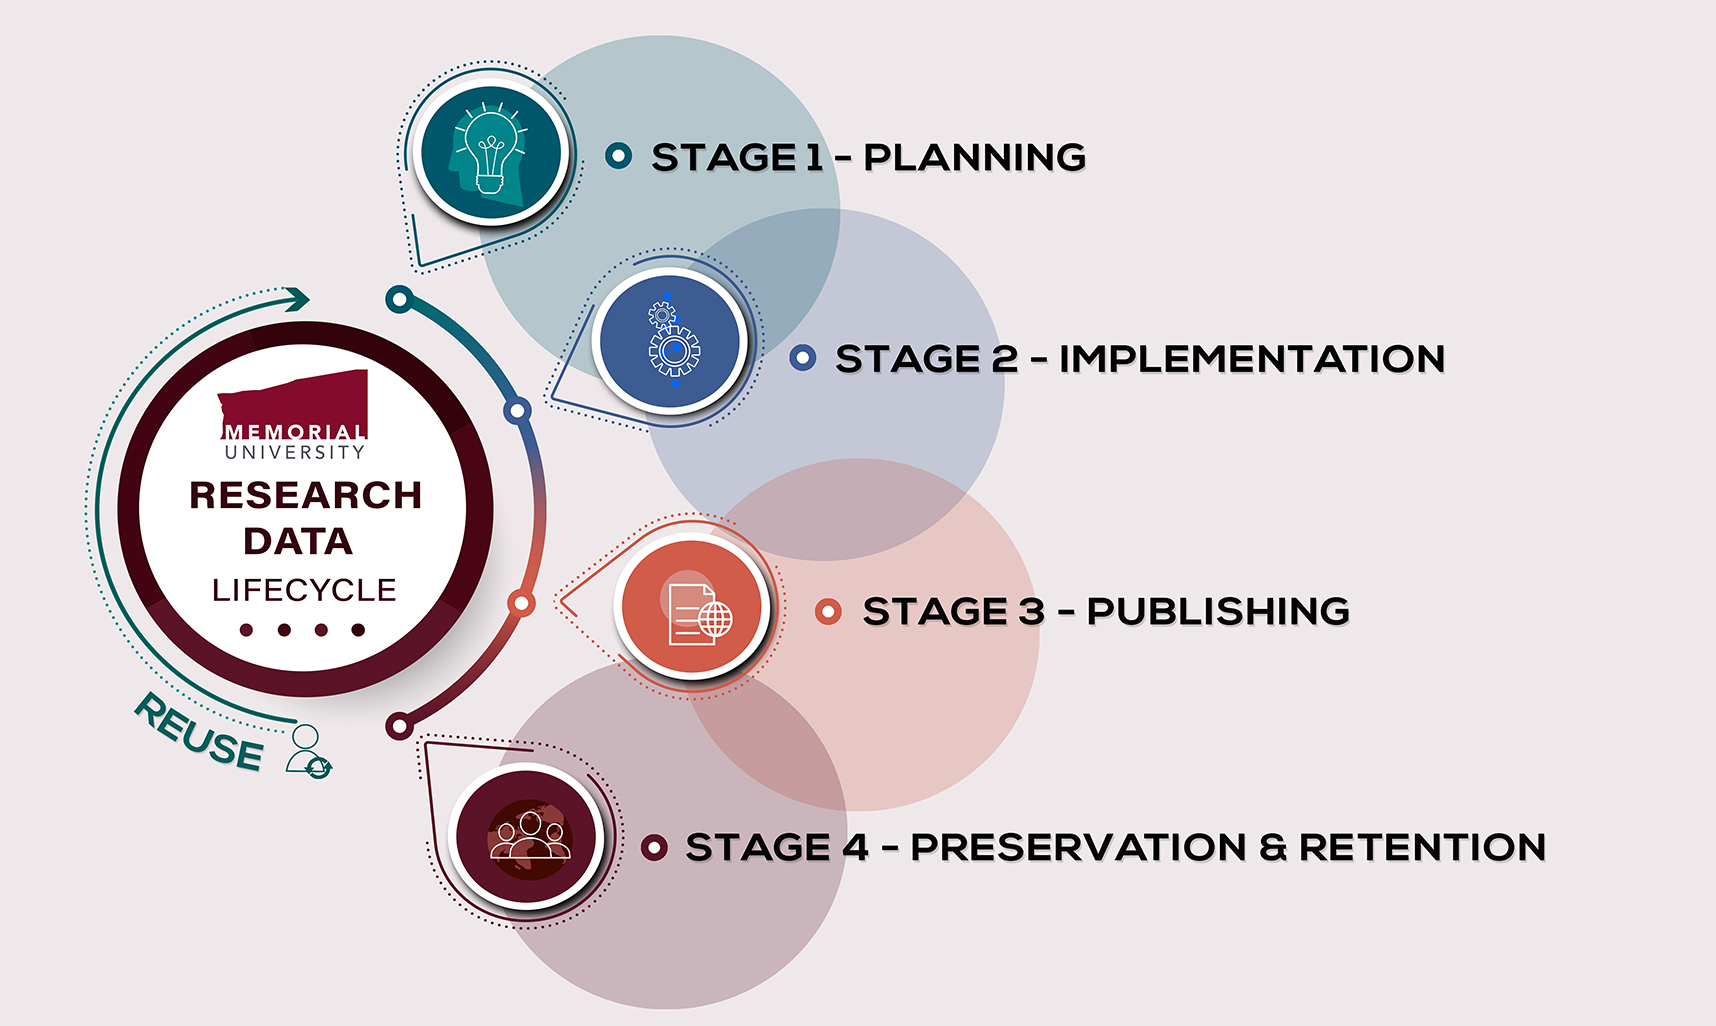
\includegraphics[keepaspectratio]{./content/research_data_lifecycle.jpg}}
\end{itemize}
\end{frame}

\begin{frame}{Étude de cas : SCS}
\phantomsection\label{uxe9tude-de-cas-scs}
\begin{itemize}
\tightlist
\item
  La Société canadienne du sang offre des données de recherche à usage
  secondaire (c'est-à-dire des bases de données sur les donneurs que
  vous pouvez demander).
\end{itemize}

Supposons que vous ayez un intérêt pour la recherche sur des données
relatives aux donneurs.

À partir des informations accessibles en ligne :

\begin{enumerate}
\tightlist
\item
  Réfléchissez à une question de recherche et évaluez si vous pourriez y
  répondre.
\item
  Décrivez le processus que vous suivriez pour obtenir les données.
\end{enumerate}

Nous reviendrons sur ces questions et verrons dans quelle mesure les
données sont FAIR
\end{frame}

\begin{frame}{Étude de cas : SCS}
\phantomsection\label{uxe9tude-de-cas-scs-1}
\begin{itemize}
\tightlist
\item
  La Société canadienne du sang offre des données de recherche à usage
  secondaire (c'est-à-dire des bases de données sur les donneurs que
  vous pouvez demander).
\end{itemize}

Supposons que vous ayez un intérêt pour la recherche sur des données
relatives aux donneurs.

À partir des informations accessibles en ligne :

\begin{enumerate}
\item
  Réfléchissez à une question de recherche et évaluez si vous pourriez y
  répondre.
\item
  Décrivez le processus que vous suivriez pour obtenir les données.
\end{enumerate}

\begin{figure}
\centering
\pandocbounded{
\includegraphics[keepaspectratio]{./content/FAIR.png}}
\caption{Fair Data Acronym}
\end{figure}
\end{frame}

\begin{frame}{Discussion}
\phantomsection\label{discussion}
\end{frame}

\begin{frame}{Données restreintes FAIR}
\phantomsection\label{donnuxe9es-restreintes-fair}
\begin{itemize}
\tightlist
\item
  \emph{F}aciles à retrouver : La découvrabilité n'a pas
  \textbf{nécessairement} besoin d'être affectée, mais elle l'est
  souvent
\item
  L'\emph{A}ccessibilité a souvent une signification différente\\
\item
  L'\emph{I}nteropérabilité peut parfois poser des problèmes
\item
  La \emph{R}éutilisabilité peut être mieux que d'ailleurs, mais cela
  demande des efforts
\end{itemize}
\end{frame}

\begin{frame}{Faciles à retrouver}
\phantomsection\label{faciles-uxe0-retrouver}
\begin{itemize}
\item
  Organisations offrant des données comme activité non prioritaire
\item
  Les ressources pour les rendre trouvables peuvent ne même pas être
  envisagées
\item
  Le savoir-faire pour rendre les données découvrables peut être
  inexistant
\item
  Même lorsqu'un ensemble de données provenant d'une source
  universitaire existe, il peut y avoir :

  \begin{enumerate}
  [a.]
  \item
    Une équipe de recherche qui utilise les données de leur côté, leur
    mise à disposition étant secondaire (voir point 1)
  \item
    Comme les données ne sont pas ouvertes, elles ne sont pas publiées,
    et les rendre trouvables demande une activité distincte (alors que
    pour les données ouvertes, elles sont souvent intégrées à un service
    qui assure à la fois leur curation et leur découvrabilité)
  \end{enumerate}
\end{itemize}
\end{frame}

\begin{frame}{Accessibles}
\phantomsection\label{accessibles}
\begin{itemize}
\tightlist
\item
  Est-ce même considéré ?
\item
  Je dirais que oui, très sérieusement, mais pas dans une optique FAIR\\
\item
  Une partie de cela est fondamentale - voir
  \href{https://doi.org/10.7191/jeslib.907}{\emph{Read et al.~2024}}
\end{itemize}
\end{frame}

\begin{frame}{Intéroperables}
\phantomsection\label{intuxe9roperables}
\begin{itemize}
\tightlist
\item
  Cela va de pair avec la découvrabilité et souffre du même problème de
  ressources.
\item
  Les métadonnées peuvent potentiellement révéler l'identité des
  individus.
\item
  Les ensembles de données restreints
  \href{https://doi.org/10.1139/facets-2023-0102}{n'ont généralement pas
  de bonnes métadonnées}
\end{itemize}
\end{frame}

\begin{frame}{Réutilsables}
\phantomsection\label{ruxe9utilsables}
\begin{itemize}
\tightlist
\item
  Les données appartiennent souvent à une organisation et ne présentent
  donc pas les mêmes risques que celles détenues par des individus.
\item
  Comme pour les problèmes d'interopérabilité et de découvrabilité, une
  mauvaise gestion des données réduit leur réutilisabilité. \#\# À quoi
  ressemble le succès ?
\end{itemize}
\end{frame}

\begin{frame}{Planification de la gestion des données}
\phantomsection\label{planification-de-la-gestion-des-donnuxe9es}
\href{https://dmp-pgd.ca/}{\emph{PGD outil de gestion}} - Pensez à ce
qui sera nécessaire à toute personne qui reprendra votre travail. Tout
ce qui vous a permis de progresser d'une étape à l'autre fait partie de
vos données de recherche. - Toutes les données du projet ne seront donc
pas restreintes, et il est important d'en tenir compte dans votre
planification.
\end{frame}

\begin{frame}{Déclarations d'accessibilité des données}
\phantomsection\label{duxe9clarations-daccessibilituxe9-des-donnuxe9es}
\begin{itemize}
\tightlist
\item
  La mention « Accès disponible sur demande » n'est PAS suffisante
\item
  Encourager la source des données à fournir un modèle pour ce type de
  formulation ! Sinon, créez-le vous-même et faites-le réviser
\end{itemize}
\end{frame}

\begin{frame}{Contenu à inclure dans une déclaration d'accessibilité des
données}
\phantomsection\label{contenu-uxe0-inclure-dans-une-duxe9claration-daccessibilituxe9-des-donnuxe9es}
\end{frame}

\begin{frame}{Contenu à inclure dans une déclaration d'accessibilité des
données}
\phantomsection\label{contenu-uxe0-inclure-dans-une-duxe9claration-daccessibilituxe9-des-donnuxe9es-1}
\begin{itemize}
\tightlist
\item
  Qui peut y accéder

  \begin{enumerate}
  [a.]
  \tightlist
  \item
    Fonction (rang) ?
  \item
    Thèmes de recherche ?
  \item
    Citoyenneté ?
  \end{enumerate}
\item
  Conditions d'accès

  \begin{enumerate}
  [a.]
  \tightlist
  \item
    Consultation ?
  \item
    Éthique ?
  \item
    Proposition de recherche ?
  \item
    Citation ?
  \item
    TRE-ERS(Trusted Research Environment / environnement de recherche
    sécurisé) ?
  \end{enumerate}
\item
  Types de licences / ententes - Ex. CC-BY (Creative Commons -- Avec
  attribution) vs.~CC-BY-NC (Creative Commons -- Avec attribution --
  Sans utilisation commerciale)
\item
  Coûts
\end{itemize}
\end{frame}

\begin{frame}{Déclaration d'accessibilité des données}
\phantomsection\label{duxe9claration-daccessibilituxe9-des-donnuxe9es}
\begin{itemize}
\tightlist
\item
  Description détaillée du processus d'accès, des critères
  d'admissibilité, avec liens vers l'information, considérations
  financières et renseignements sur la licence ou les conditions
  d'utilisation.
\end{itemize}
\end{frame}

\begin{frame}{Efforts de découverte des données}
\phantomsection\label{efforts-de-duxe9couverte-des-donnuxe9es}
\begin{itemize}
\tightlist
\item
  Toute source de données peut désormais être indexée relativement
  facilement dans Lunaris.
\item
  Dépôts réservés aux métadonnées lorsqu'il y a des informations à
  fournir aux utilisateurs potentiels.
\item
  Les dépôts réservés aux métadonnées créent également un identifiant
  persistant (PID), ce qui rend les données beaucoup plus faciles à
  trouver pour quelqu'un qui souhaite les utiliser ultérieurement, car
  \href{https://guides.library.oregonstate.edu/research-data-services/data-management-data-citation}{\emph{VOUS
  POUVEZ LES CITER}}
\end{itemize}
\end{frame}

\begin{frame}{Efforts de préservation}
\phantomsection\label{efforts-de-pruxe9servation}
\begin{itemize}
\item
  Si une source de données écrase mes données avec une nouvelle copie
  sans l'indiquer, toute personne cherchant à reproduire mon travail
  sera au mieux très confuse.
\item
  Idéalement, les nouvelles versions devraient avoir de nouveaux
  identifiants persistants (PID), et les anciennes versions devraient
  renvoyer vers la plus récente, ou bien tout devrait être regroupé sous
  un seul PID avec une gestion des versions.
\item
  La fréquence de suivi des versions dépendra de la fréquence d'accès et
  des préférences des organisations. \#\# Comment en discuter avec la
  source de mes données\,?
\item
  Soulever la question
\item
  Mettre en évidence les avantages de recourir à de telles pratiques
\item
  Diriger vers les ressources disponibles
\end{itemize}
\end{frame}

\begin{frame}{Étude de cas : indexation dans Lunaris}
\phantomsection\label{uxe9tude-de-cas-indexation-dans-lunaris}
\begin{itemize}
\tightlist
\item
  Lunaris est un service de l'Alliance de recherche numérique du Canada
\item
  Ce service regroupe les métadonnées provenant de diverses sources
\item
  Les fournisseurs de données peuvent collaborer avec Lunaris pour faire
  indexer leurs ensembles de données
\end{itemize}
\end{frame}

\begin{frame}{Lunaris page}
\phantomsection\label{lunaris-page}
\begin{figure}
\centering
\pandocbounded{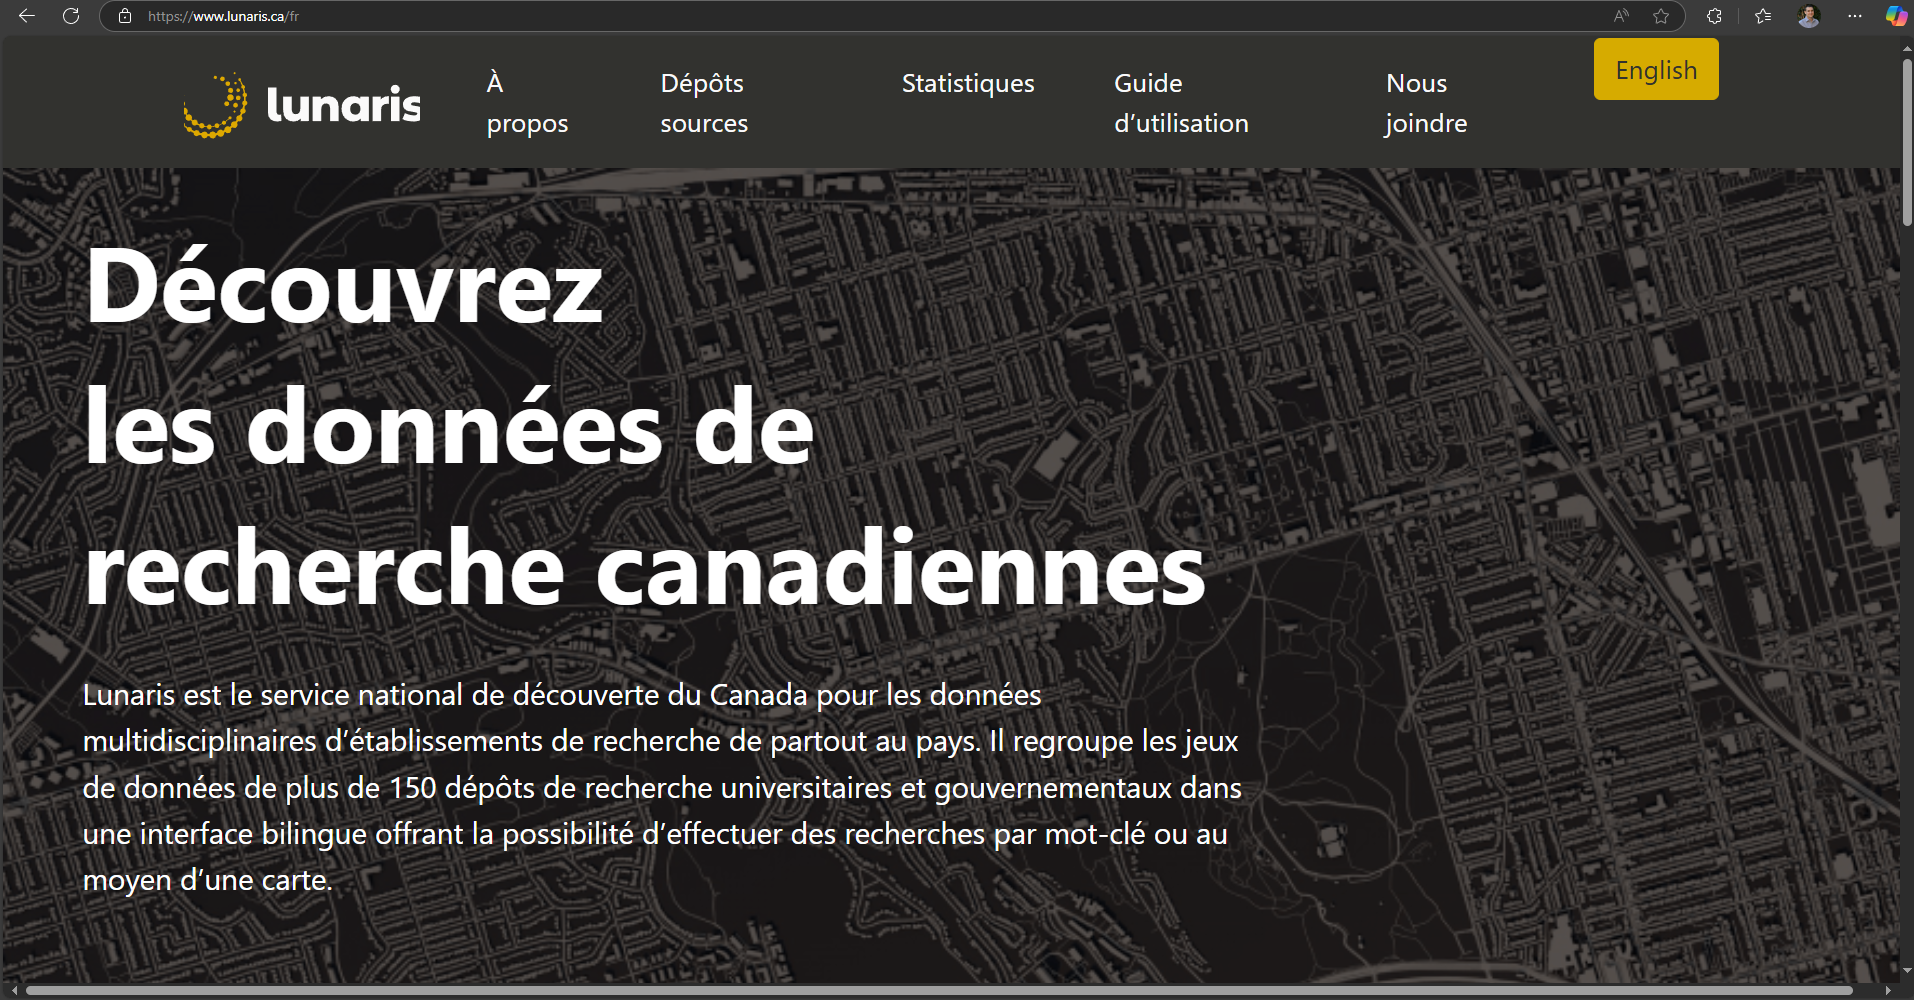
\includegraphics[keepaspectratio]{./content_fr/lunaris.png}}
\caption{Lunaris webpage screenshot}
\end{figure}
\end{frame}

\begin{frame}{Exigences du système}
\phantomsection\label{exigences-du-systuxe8me}
\begin{itemize}
\tightlist
\item
  Lunaris dispose d'un schéma de métadonnées (liste des informations
  qu'il peut traiter et afficher).
\item
  Toute source de données peut fournir une base de données contenant ces
  informations sur ses jeux de données pour qu'elles soient «
  moissonnées ».
\item
  Collaborer avec l'équipe de Lunaris pour déterminer le format des
  données (exemples issus de notre étude de cas disponibles dans le
  dossier de l'atelier).
\end{itemize}
\end{frame}

\begin{frame}{Étude de cas}
\phantomsection\label{uxe9tude-de-cas}
\begin{figure}
\centering
\pandocbounded{
\includegraphics[keepaspectratio]{./content_fr/CRDCN_screenshot.jpg}}
\caption{\emph{CRDCN data webpage screenshot}}
\end{figure}
\end{frame}

\begin{frame}{Étude de cas}
\phantomsection\label{uxe9tude-de-cas-1}
\begin{figure}
\centering
\pandocbounded{
\includegraphics[keepaspectratio]{./content_fr/CRDCN_screenshot_hlt.jpg}}
\caption{CRDCN webpage data screenshot}
\end{figure}
\end{frame}

\begin{frame}{Étude de cas}
\phantomsection\label{uxe9tude-de-cas-2}
\begin{figure}
\centering
\pandocbounded{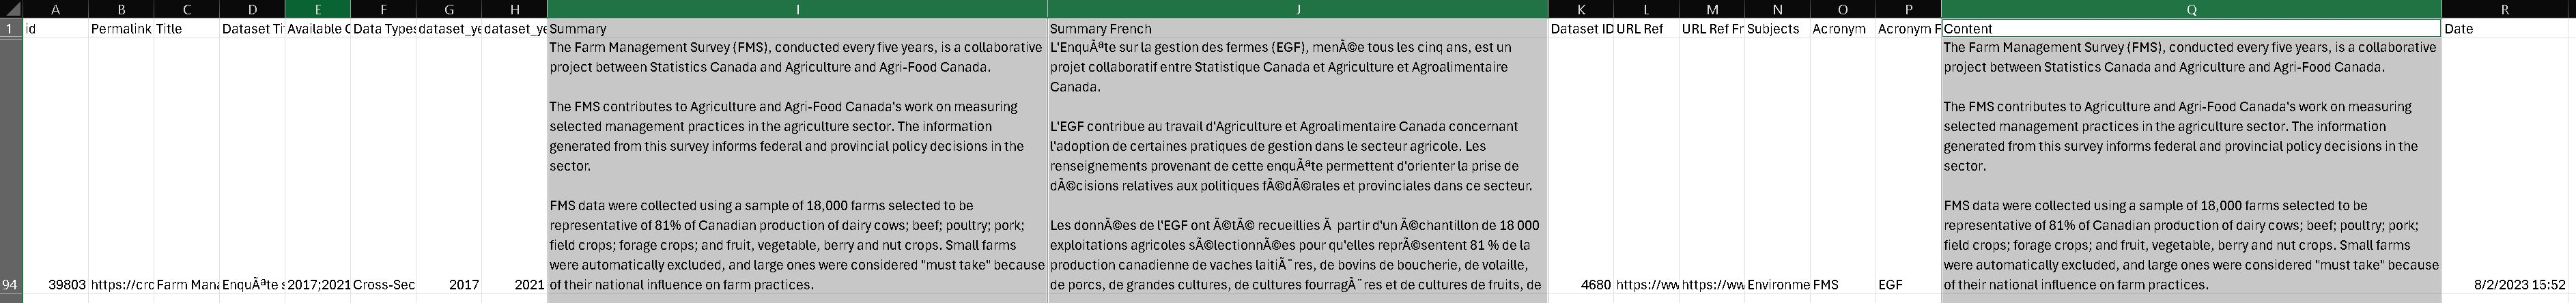
\includegraphics[keepaspectratio]{./content_fr/DB screenshot.jpg}}
\caption{Screenshot of CRDCN dataset database}
\end{figure}
\end{frame}

\begin{frame}{Étape 1 : Correspondance des métadonnées}
\phantomsection\label{uxe9tape-1-correspondance-des-muxe9tadonnuxe9es}
\begin{itemize}
\tightlist
\item
  Plus simple qu'il n'y paraît\\
\item
  Faire correspondre les champs de ma base de données avec le schéma de
  Lunaris
\item
  Dans certains cas, ces champs seront remplis automatiquement et
  faciles à repérer (ex. ``Nom de la base de données'').\\
\item
  Certains seront dynamiques et moins évidents.
\item
  Dans certains cas, ils seront statiques et devront être créés
  manuellement (ex. ``Droits'').
\end{itemize}
\end{frame}

\begin{frame}{Exemples de correspondances}
\phantomsection\label{exemples-de-correspondances}
\begin{itemize}
\tightlist
\item
  Sujets + champs statiques -\textgreater{} Mots-clés
\item
  Paramètres d'accès (statique) -\textgreater{} License
\item
  Lien permanent (crdcn.ca) -\textgreater{} URL
\item
  Identifiant du catalogue -\textgreater{} Identifiant
\end{itemize}
\end{frame}

\begin{frame}{Étape 2 : Code de traduction}
\phantomsection\label{uxe9tape-2-code-de-traduction}
\begin{itemize}
\tightlist
\item
  Exemple dans les ressources (.py et .R) pour nos traductions
\item
  Champs dynamiques mis en correspondance avec la base de données
  actuelle
\item
  Champs statiques ajoutés à la fin
\item
  Si vous avez des métadonnées EN/FR, les deux devraient figurer dans un
  seul fichier
\item
  Écrire la sortie dans un fichier .json
\end{itemize}
\end{frame}

\begin{frame}{Étape 3 : Publier}
\phantomsection\label{uxe9tape-3-publier}
\begin{itemize}
\tightlist
\item
  Publiez le fichier .json à un endroit accessible sur le web (n'importe
  où) et partagez-le avec l'équipe de Lunaris.
\item
  Les mises à jour apportées au fichier se réflèteront automatiquement
  dans Lunaris (l'outil de collecte (« harvester ») revérifie
  périodiquement).
\end{itemize}
\end{frame}

\begin{frame}{Résultat}
\phantomsection\label{ruxe9sultat}
\begin{itemize}
\tightlist
\item
  Un ensemble de données restreint devient beaucoup plus facile à
  repérer pour celles et ceux qui recherchent de l'information sur un
  sujet donné.
\item
  Les mises à jour des métadonnées, y compris les protocoles d'accès,
  les informations sur l'ensemble de données et même les nouvelles
  données disponibles, sont interprétables par un système informatique.
  \#\# Résultat
\end{itemize}

\href{https://test.lunaris.ca/catalog/87dc478c-8d31-5d5f-8394-ce8c8d5f9448?locale=fr&q=&f\%5Bfrdr_origin_id\%5D\%5B\%5D=CRDCN}{\emph{Example}}
\end{frame}

\begin{frame}{Option 2 -- Dépôts de métadonnées uniquement}
\phantomsection\label{option-2-duxe9puxf4ts-de-muxe9tadonnuxe9es-uniquement}
\begin{itemize}
\tightlist
\item
  Plus détaillés et plus utiles pour les autres
\item
  Génèrent un profil de métadonnées similaire à l'exemple précédent
\item
  MAIS, ils peuvent inclure de la documentation
\end{itemize}
\end{frame}

\begin{frame}{Présentation : Boréalis}
\phantomsection\label{pruxe9sentation-boruxe9alis}
\begin{itemize}
\tightlist
\item
  Ensemble national d'instances Dataverse (provenant de la plupart des
  universités canadiennes)
\item
  Votre Dataverse intègre les données, et Borealis les regroupe dans un
  service national
\item
  Les informations de Borealis sont collectées par d'autres outils de
  recherche (y compris Lunaris)
\item
  \href{https://demo.borealisdata.ca/dataset.xhtml?persistentId=doi\%3A10.80240\%2FFK2\%2FDTCL3Z&version=DRAFT}{\emph{Exemple}}
\end{itemize}
\end{frame}

\begin{frame}{Boréalis et données à accès restreint}
\phantomsection\label{boruxe9alis-et-donnuxe9es-uxe0-accuxe8s-restreint}
\begin{itemize}
\tightlist
\item
  Can't deposit personally identifiable info into Borealis
\item
  CAN create metadata records including deposit of supporting documents
\item
  With the right supporting documents, Borealis can be a very effective
  tool for data discovery

  \begin{itemize}
  \tightlist
  \item
    Anonymized version of dataset
  \item
    Questionnaires
  \item
    Structural files
  \end{itemize}
\end{itemize}
\end{frame}

\begin{frame}{Boréalis et données à accès restreint}
\phantomsection\label{boruxe9alis-et-donnuxe9es-uxe0-accuxe8s-restreint-1}
\begin{itemize}
\tightlist
\item
  Métadonnées seules \textless{} Métadonnées avec documents sommaires
  \textless{} Métadonnées avec information au niveau des variables
\item
  Un document de référence et un guide explicatif sont disponibles
\end{itemize}
\end{frame}

\begin{frame}{Pourquoi choisir Boréalis vs Lunaris}
\phantomsection\label{pourquoi-choisir-boruxe9alis-vs-lunaris}
Avantages de Lunaris :

\begin{itemize}
\tightlist
\item
  Mises à jour du contenu dynamiques et automatiques
\item
  Effort minimal pour créer une série d'entrées à partir de données
  existantes
\end{itemize}

Avantages de Borealis :

\begin{itemize}
\tightlist
\item
  Offre un niveau de détail accru sur la ressource
\item
  Autorise le dépôt de documents
\item
  Crée une page de destination permanente pour la ressource
\item
  Attribue un DOI à la ressource, assorti d'un suivi des versions
\end{itemize}
\end{frame}

\begin{frame}{Pourquoi choisir Boréalis vs Lunaris}
\phantomsection\label{pourquoi-choisir-boruxe9alis-vs-lunaris-1}
Lunaris -- Inconvénients

\begin{itemize}
\tightlist
\item
  Informations limitées et peu flexibles sur la source des données
\item
  Nécessite une page de renvoi vers laquelle diriger les gens qui
  veulent consulter l'information
\item
  Aucune permanence du dossier : rien n'est créé pour être cité ou
  référencé
\item
  Le système exige certaines compétences techniques pour alimenter ou
  naviguer automatiquement
\end{itemize}

Borealis -- Inconvénients - Processus de création ou de mise à jour des
fiches est plus complexe - De nombreux champs à remplir (même si la
plupart sont facultatifs) - Les fiches ne peuvent pas être supprimées
(ce qui peut aussi être un avantage) - L'accès pour téléverser est
réservé aux membres du consortium
\end{frame}

\begin{frame}{Quand utiliser Lunaris}
\phantomsection\label{quand-utiliser-lunaris}
\begin{itemize}
\tightlist
\item
  Série de pages de destination préexistantes et établies
\item
  Aucune documentation supplémentaire à téléverser
\item
  Modifications, ajouts ou mises à jour fréquents qui ne reflètent pas
  de changements dans les données sous-jacentes
\item
  Fournisseur de données qui n'est pas membre du consortium
\end{itemize}
\end{frame}

\begin{frame}{Quand utiliser Borealis}
\phantomsection\label{quand-utiliser-borealis}
\begin{itemize}
\tightlist
\item
  Vous souhaitez attribuer un identifiant pérenne (PID) à l'ensemble de
  données
\item
  Vous avez des informations contextuelles supplémentaires à fournir
  (ex. : téléversement de fichiers PDF, métadonnées plus détaillées)
\end{itemize}
\end{frame}

\begin{frame}{Merci de votre attention}
\phantomsection\label{merci-de-votre-attention}
\begin{itemize}
\item
  Questions ?
\item
  \href{mailto:grant.gibson@crdcn.ca}{\nolinkurl{grant.gibson@crdcn.ca}}
\end{itemize}
\end{frame}

\end{document}
